\documentclass[border=5pt]{standalone}
\usepackage[T1]{fontenc}
\usepackage{tikz}

\definecolor{garnet}{HTML}{73000A}
\definecolor{atlantic}{HTML}{466A9F}
\definecolor{congaree}{HTML}{1F414D}
\definecolor{warmgrey}{HTML}{676156}
\definecolor{bk70}{HTML}{5C5C5C}
\definecolor{bk30}{HTML}{C7C7C7}
\definecolor{bk10}{HTML}{ECECEC}

\begin{document}
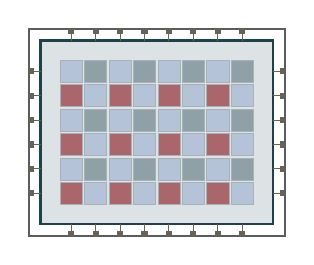
\begin{tikzpicture}

  % === CMOS Sensor — front view ===
  % Based on test_stereo.tex pixel grid, scaled up to standalone component

  \def\npx{8}        % pixels per row
  \def\npy{6}        % pixels per column
  \def\pxsize{0.28}  % pixel pitch
  \def\gap{0.03}     % gap between pixels

  % Substrate (die) — slightly larger than pixel array
  \pgfmathsetmacro{\arrayW}{\npx * \pxsize + (\npx - 1) * \gap}
  \pgfmathsetmacro{\arrayH}{\npy * \pxsize + (\npy - 1) * \gap}
  \pgfmathsetmacro{\pad}{0.25}
  \pgfmathsetmacro{\dieW}{\arrayW + 2*\pad}
  \pgfmathsetmacro{\dieH}{\arrayH + 2*\pad}

  % Die background
  \fill[congaree!15] (-\pad, -\pad) rectangle (\arrayW + \pad, \arrayH + \pad);
  \draw[congaree, thick] (-\pad, -\pad) rectangle (\arrayW + \pad, \arrayH + \pad);

  % Pixel array — Bayer-like color pattern
  \foreach \ix in {0,...,7} {
    \foreach \iy in {0,...,5} {
      \pgfmathsetmacro{\px}{\ix * (\pxsize + \gap)}
      \pgfmathsetmacro{\py}{\iy * (\pxsize + \gap)}
      % Bayer pattern: RGGB
      \pgfmathsetmacro{\iseven}{mod(\ix + \iy, 2)}
      \pgfmathsetmacro{\isGreenRow}{mod(\iy, 2)}
      % Row even + col even = R, row even + col odd = G
      % Row odd + col even = G, row odd + col odd = B
      \pgfmathtruncatemacro{\rowmod}{mod(\iy, 2)}
      \pgfmathtruncatemacro{\colmod}{mod(\ix, 2)}
      \ifnum\rowmod=0
        \ifnum\colmod=0
          % Red pixel
          \fill[garnet!60] (\px, \py) rectangle (\px + \pxsize, \py + \pxsize);
          \draw[congaree!40, very thin] (\px, \py) rectangle (\px + \pxsize, \py + \pxsize);
        \else
          % Green pixel
          \fill[atlantic!40] (\px, \py) rectangle (\px + \pxsize, \py + \pxsize);
          \draw[congaree!40, very thin] (\px, \py) rectangle (\px + \pxsize, \py + \pxsize);
        \fi
      \else
        \ifnum\colmod=0
          % Green pixel
          \fill[atlantic!40] (\px, \py) rectangle (\px + \pxsize, \py + \pxsize);
          \draw[congaree!40, very thin] (\px, \py) rectangle (\px + \pxsize, \py + \pxsize);
        \else
          % Blue pixel
          \fill[congaree!50] (\px, \py) rectangle (\px + \pxsize, \py + \pxsize);
          \draw[congaree!40, very thin] (\px, \py) rectangle (\px + \pxsize, \py + \pxsize);
        \fi
      \fi
    }
  }

  % Wire bonds — short lines from die edge to package
  \pgfmathsetmacro{\pkgpad}{0.15}
  % Bottom bonds
  \foreach \ix in {0,...,7} {
    \pgfmathsetmacro{\bx}{\ix * (\pxsize + \gap) + \pxsize/2}
    \draw[warmgrey, thin] (\bx, -\pad) -- (\bx, -\pad - \pkgpad);
  }
  % Top bonds
  \foreach \ix in {0,...,7} {
    \pgfmathsetmacro{\bx}{\ix * (\pxsize + \gap) + \pxsize/2}
    \draw[warmgrey, thin] (\bx, \arrayH + \pad) -- (\bx, \arrayH + \pad + \pkgpad);
  }
  % Left bonds
  \foreach \iy in {0,...,5} {
    \pgfmathsetmacro{\by}{\iy * (\pxsize + \gap) + \pxsize/2}
    \draw[warmgrey, thin] (-\pad, \by) -- (-\pad - \pkgpad, \by);
  }
  % Right bonds
  \foreach \iy in {0,...,5} {
    \pgfmathsetmacro{\by}{\iy * (\pxsize + \gap) + \pxsize/2}
    \draw[warmgrey, thin] (\arrayW + \pad, \by) -- (\arrayW + \pad + \pkgpad, \by);
  }

  % Package outline
  \pgfmathsetmacro{\pkgW}{\dieW + 2*\pkgpad}
  \pgfmathsetmacro{\pkgH}{\dieH + 2*\pkgpad}
  \draw[bk70, thick] (-\pad - \pkgpad, -\pad - \pkgpad)
    rectangle (\arrayW + \pad + \pkgpad, \arrayH + \pad + \pkgpad);

  % Bond pads (small squares at wire bond ends on package edge)
  \foreach \ix in {0,...,7} {
    \pgfmathsetmacro{\bx}{\ix * (\pxsize + \gap) + \pxsize/2}
    \fill[warmgrey] (\bx - 0.04, -\pad - \pkgpad) rectangle (\bx + 0.04, -\pad - \pkgpad + 0.06);
    \fill[warmgrey] (\bx - 0.04, \arrayH + \pad + \pkgpad - 0.06) rectangle (\bx + 0.04, \arrayH + \pad + \pkgpad);
  }
  \foreach \iy in {0,...,5} {
    \pgfmathsetmacro{\by}{\iy * (\pxsize + \gap) + \pxsize/2}
    \fill[warmgrey] (-\pad - \pkgpad, \by - 0.04) rectangle (-\pad - \pkgpad + 0.06, \by + 0.04);
    \fill[warmgrey] (\arrayW + \pad + \pkgpad - 0.06, \by - 0.04) rectangle (\arrayW + \pad + \pkgpad, \by + 0.04);
  }

\end{tikzpicture}
\end{document}
